\documentclass[BoSSSForSolvingConservationLaws.tex]{subfiles}

\begin{document}

\subsection{Transformation to physical domain}
Referring to equation \eqref{WeakFormulation-BoSSSStyle} we need to calculate integrals on $K_j$ and $\partial K_j$. In order not to perform these integrations for all elements of the grid we integrate on a reference domain (reference element) $K_{ref}$ and then transform to physical domain. To know about the reference elements see \cite{KummerLayer2Manual09}. Here we use an affine-linear transformation $T_j$.
\[
\vec{x}=T_j(\grvec{\upxi})=M_j\grvec{\upxi}+\vec{a}_j
\]
$M_j$\nomenclature{$M_j$}{Matrix of transformation to physical domain for cell j} is a linear matrix which accounts for stretching, rotation or shear and $\vec{a}_j$ performs a translation. As centroid of a reference element is chosen to be zero, $\vec{a}_j$ would be centroid of each cell $j$. Result of this transformation is that element $j$ is scaled by $|det(M_j)|$.
\begin{align*}
  &\int_{K_j} d\vec{x}=|det(M_j)|\int_{K_{ref}} d\vec{\upxi}\\
  &\nabla_{\vec{x}}=((M_j)^{-1})^T \nabla_{\vec{\upxi}}
\end{align*}
The orthonormal polynomial $\phi_{jn}$ defined on element $j$ in physical domain is related to $\phi_n$ orthonormal polynomial on reference element (see section \ref{sec:Polynomials}) by\\
\begin{align*}
  &\phi_{jn}(\vec{x})=\frac{1}{\sqrt{|det(M_j)|}}\phi_n(\grvec{\upxi})\\
  &\nabla_{\vec{x}} \phi_{jn}(\vec{x})=\frac{1}{\sqrt{|det(M_j)|}} ((M_j)^{-1})^T \nabla_{\grvec{\upxi}} \phi_n(\grvec{\upxi})
\end{align*}

\begin{comment}
Therefore the stiffness matrices and fluxes are\\
\begin{align*}
&{S_{jmn}^l}=\frac{1}{|det(M_j)|} ((M_j)^{-1})^T \int_{K_{ref}} \phi_{jm}(\grvec{\upxi}) \frac{\partial \phi_{jn}(\grvec{\upxi})}{\partial {\xi}_l} d(\grvec{\upxi}), \qquad 1\leq m,n \leq N_p \\
&F_{jm}^*=\frac{1}{\sqrt{|det(M_j)|}} \oint_{K_{ref}} \hat{n}\cdot \vec{f}^* \phi_j(\grvec{\upxi}) d(\grvec{\upxi}), \qquad 1\leq m \leq N_p
\end{align*}
For integrating the stiffness matrices and fluxes on reference elements we use Gaussian quadrature rules.
\end{comment}

\subsubsection*{Implementation in BoSSS}
Matrices $M_j$ and $(M_j)^{-1}$ of all cells of domain are stored as 2D arrays called \emph{transformation}\coderm{BoSSS.Foundation.Grid.GridData.Transformation} and \emph{inverse transformation}\coderm{BoSSS.Foundation.Grid.GridData.InverseTransformation}. Vector $\vec{a}_j$ is \emph{affine offset}\coderm{BoSSS.Foundation.Grid.GridData.AffineOffset}. The scaling factors $|det(M_j)|$\coderm{BoSSS.Foundation.Grid.GridData.AbsDetTransformation} and $\frac{1}{\sqrt{|det(M_j)|}}$\coderm{BoSSS.Foundation.Grid.GridData.OneOverSqrt\_AbsDetTransformation} are available for each cell $j$. For edges scaling factors $|det(M_i)|$\coderm{BoSSS.Foundation.Grid.GridData.AbsDetEdgeTransformation} are stored. $M_i$ would be transformation matrix for edge $i$\nomenclature{$i$}{Edge index} but it's not stored.

\subsubsection*{Inter-cell transformation}
When we integrate on edges of reference elements, we need values of the fields in physical domain to calculate numerical fluxes. To do so, points from edge simplex coordinate system must be transferred\coderm{BoSSS.Foundation.Grid.Simplex.TransformEdgeCoordinates(...)} to volume simplex coordinates and then to physical coordinates. Consider edge $i$ in figure \ref{fig:InterCellTransformation}, its first neighbor cell $j$ and its second neighbor cell $j'$\nomenclature{$j'$}{Index of second neighbor cell of edge $i$}. Let's say that the grid generator has stored edges of elements in a counter clockwise order. Each point of the edge $i$ in physical domain has different coordinates in both volume simplex and edge simplex coordinate systems shown by $\Box$ for cell $j$ and $\times$ for cell $j'$. Therefore if we only choose point $\Box$ in edge simplex coordinate system and transform to volume and physical coordinates, the transformation doesn't result in point $\times$ in the second neighbor. In order to avoid this problem, by having the coordinates of point $\Box$ in volume simplex we find point $\times$ using \emph{inter-cell transformations}\coderm{BoSSS.Foundation.Grid.GridData.InterCellTransformations}, before transforming to physical domain. Inter-cell transformations is an array of all transformations found for a specific grid. Index to this array is stored\coderm{BoSSS.Foundation.Grid.GridData.TrafoTo2ndCell} for each edge $i$.
\begin{figure}[h]
\begin{center}
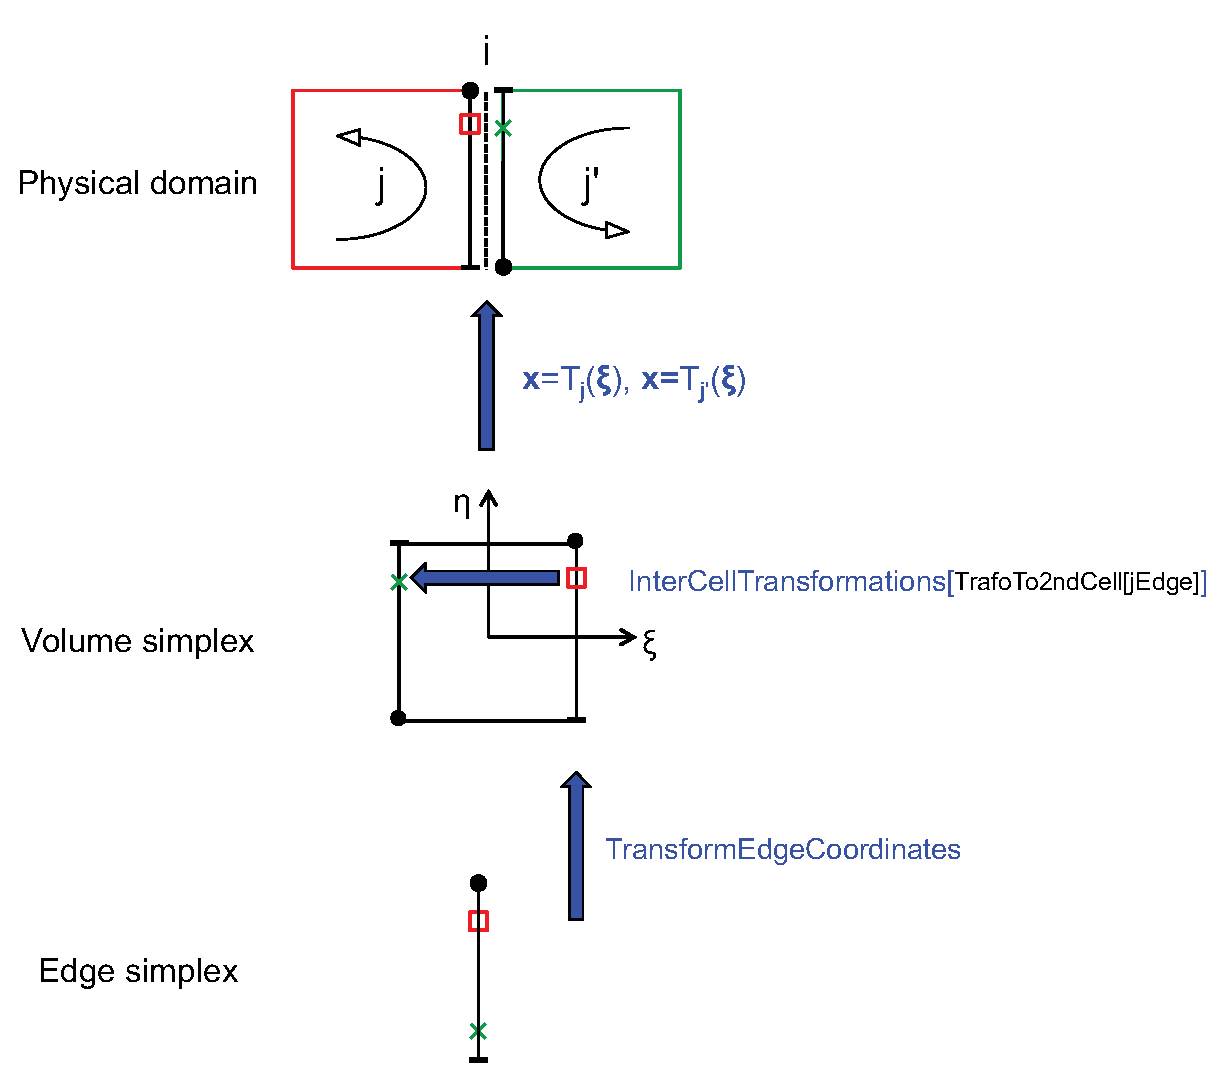
\includegraphics[width=13cm]{Figures/InterCellTransformation}
\end{center}
\caption{Relation between physical, volume simplex and edge simplex coordinate systems}
\label{fig:InterCellTransformation}
\end{figure}

\subsection{Specifying some points inside a volume simplex}
In many occasions you may think about doing some operations (like integration, evaluation of a field,...) at some points inside elements. As it is described above such operations are done in the reference elements and then transformation is made to physical domain. Therefore we specify the points in the volume simplex coordinate system and create\coderm{BoSSS.Foundation.NodeSetController.CreateContainer(...)} a \emph{node set container}\coderm{BoSSS.Foundation.NodeSetController.NodeSetContainer} out of them which contains the desired points as a \emph{node set}\coderm{BoSSS.Foundation.NodeSetController.NodeSetContainer.NodeSet}. An array of some node set containers is called a \emph{node set family} and then the node sets are accessed with an index called \emph{node set index}.

\end{document} 